\section{Theorie}
\label{sec:Theorie}

Brückenschaltungen sind eine präzise Methode in der Messtechnik, um unbekannte Impedanzen zu vermessen.
Sie werden auch zur Bestimmung von pyhsikalischen Größen benutzt, die sich über eine Impedanz identifizieren lassen, wie zum Beispiel die Temperatur.
Die hier behandelten Schaltungen sind abgeglichene Brücken, die auf der Nullmethode basieren.
Eine allgemeine Brückenschaltung ist in Abblidung \ref{fig:Schaltung1} zu sehen.
\begin{figure}
  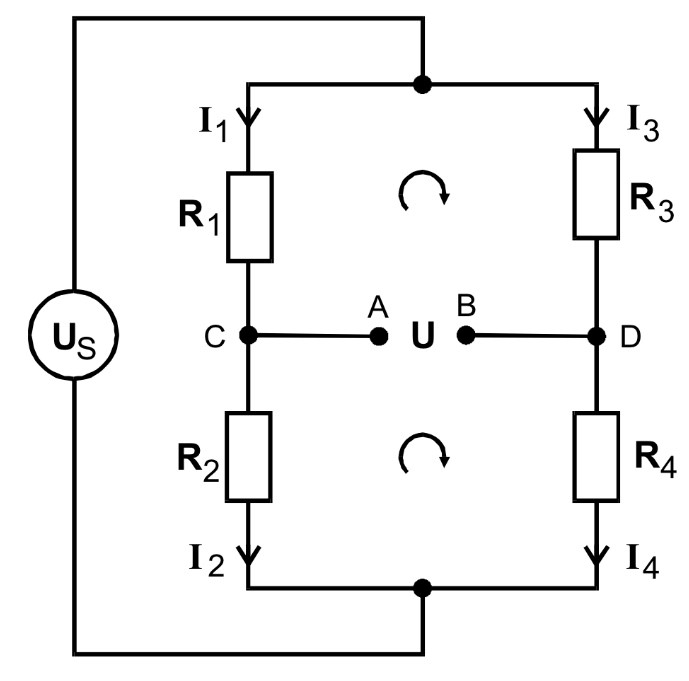
\includegraphics[height=6cm]{data/Schaltung1.jpg}
  \centering
  \caption{Allgemeine Brückenschaltung.}
  \label{fig:Schaltung1}
\end{figure}
An eine Masche, die in 2 weitere Maschen aufegteilt werden kann, ist eine äußere Speisespannung $U_{\text{s}}$ angelegt.
Gemessen wird die Spannung zwischen Punkt A und B, die als Brückenspannung bezeichnet wird und vom Verhältnis der Impedanzen abhängt.
Bei der Nullmethode wird eine unbekannte Impedanz gemessen, indem das Verhältnis der restlichen bekannten Impedanzen so variiert, dass die Brückenspannung Null wird.
Mit Hilfe der Kirchhoffschen Regeln
\begin{itemize}
  \item \textcquote{V302}{1. In einem Verzweigungspunkt von elektrischen Strömen [...] ist die Summe der zufließenden Ströme ($\symbf{I}$ > 0) gleich der Summe der abfließenden Ströme ($\symbf{I}$ < 0).}
  \item \textcquote{V302}{2. in jedem beliebig aus einem Leiternetzwerk herausgegriffenen, in sich geschlossenen Stromkreis (\enquote{Masche}) ist die Summe der elektromotorischen Kräfte [...] gleich der Summe der Produkte aus den Stromstärken und den Widerständen [...].}
\end{itemize}
kann berechnet werden, für welche Verhältnisse der Impedanzen der Zustand einer verschwindenden Brückenspannung auftritt.
Ist eine Impedanz gegeben als komplexe Zahl $\symbffrak{Z} = X + \text{i}Y$, muss gelten:
\begin{equation}
  \symbffrak{Z}_1 \symbffrak{Z}_4 = \symbffrak{Z}_2 \symbffrak{Z}_3
  \label{eqn:gl1}
\end{equation}
Also müssen Imaginär- und Realteil gleich sein:
\begin{equation}
  X_1 X_4 - Y_1 Y_4 = X_2 X_3 - Y_2 Y_3 \\
  \label{eqn:gl2}
\end{equation}
\begin{equation}
  X_1 Y_4 + X_4 Y_1 = X_2 Y_3 + X_3 Y_2
  \label{eqn:gl3}
\end{equation}
Daraus kann dann auf die Impedanz des unbekannten Bauteils geschlossen werden.
Im Folgenden wird auf verschiedene Brückenschaltungen im Einzelnen eingegangen.

\subsection{Wheatstonesche Brücke}
\label{sec:Theorie1}
Die in Abbildung \ref{fig:Schaltung2} dargestellte Schaltung setzt sich nur aus ohmschen Widerständen zusammen, kann also mit Gleich- und Wechselstrom betrieben werden.
Sie kann dazu genutzt werden, um einen unbekannten Widerstand $R_x$ zu ermitteln.
\begin{equation}
  R_x = R_2 \frac{R_3}{R_4}
  \label{eqn:gl4}
\end{equation}
\begin{figure}
  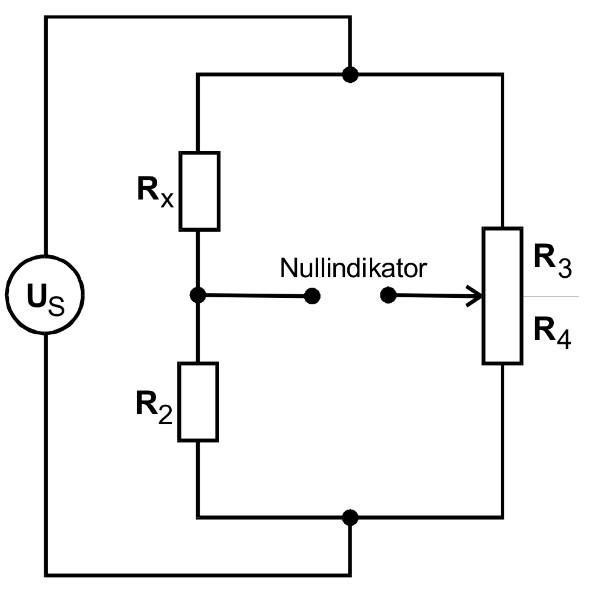
\includegraphics[height=6cm]{data/Schaltung2.jpg}
  \centering
  \caption{Wheatstonesche Brückenschaltung.}
  \label{fig:Schaltung2}
\end{figure}
\FloatBarrier

\subsection{Kapazitätsmessbrücke}
\label{sec:Theorie2}
Ein reeler Kondensator besitzt neben seiner Kapazität, auch immer einen ohmschen Widerstand, die beide mit der Brücke in Abbildung \ref{fig:Schaltung3} bestimmt werden können.
Hierfür sind zwei Abstimmungsfreiheitsgerade notwendig, da die Brückenspannung nach Betrag und Phase verschwinden muss für die Erfüllung von \eqref{eqn:gl2} und \eqref{eqn:gl3}.
\begin{equation}
  R_x = R_2 \frac{R_3}{R_4}
  \label{eqn:gl5}
\end{equation}
\begin{equation}
  C_x = C_2 \frac{R_4}{R_3}
  \label{eqn:gl6}
\end{equation}
\begin{figure}
  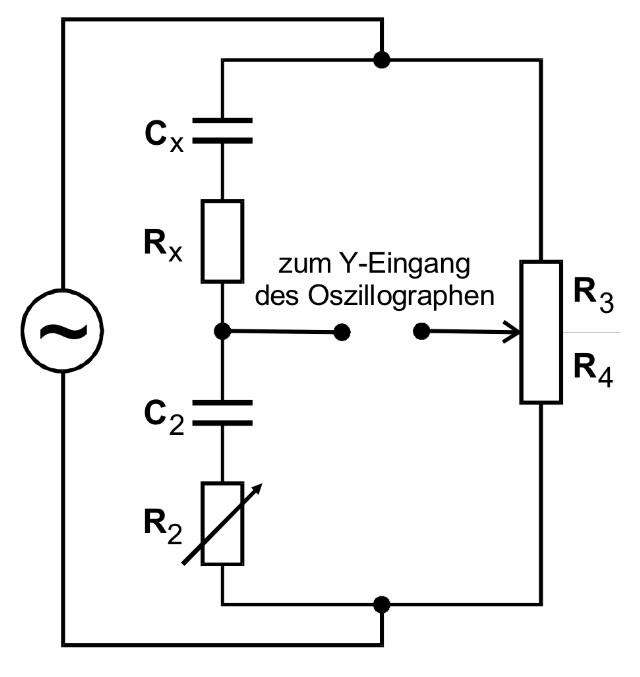
\includegraphics[height=6cm]{data/Schaltung3.jpg}
  \centering
  \caption{Messbrücke für verlustbehaftete Kapazitäten.}
  \label{fig:Schaltung3}
\end{figure}
\FloatBarrier

\subsection{Induktivitätsmessbrücke}
\label{sec:Theorei3}
Auch eine Spule besitzt einen ohmschen Widerstand, zusätzlich zu ihrer Induktivität.
Eine Schaltung wie in Abbildung \ref{fig:Schaltung4} ermöglicht die Vermessung der Spule.
\begin{equation}
  R_x = R_2 \frac{R_3}{R_4}
  \label{eqn:gl7}
\end{equation}
\begin{equation}
  L_x = L_2 \frac{R_3}{R_4}
  \label{eqn:gl8}
\end{equation}
\begin{figure}
  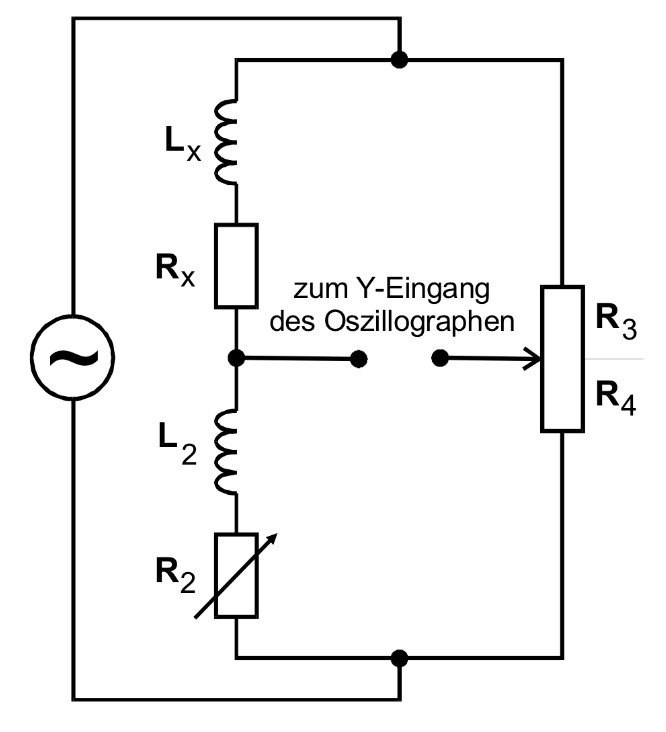
\includegraphics[height=6cm]{data/Schaltung4.jpg}
  \centering
  \caption{Messbrücke für verlustbehaftete Induktivitäten.}
  \label{fig:Schaltung4}
\end{figure}
\FloatBarrier

\subsection{Maxwell-Brücke}
\label{sec:Theorie4}
Die Maxwell-Brücke dient ebenfalls der Messung einer verlustbehafteten Spule, die bekannte Induktivität $L_2$ wird jedoch durch Kapazität $C_2$ ersetzt (vergleiche Abb. \ref{fig:Schaltung4} und \ref{fig:Schaltung5}).
Folgende Bedingungen gelten für diese Schaltung:
\begin{equation}
  R_x = \frac{R_2 R_3}{R_4}
  \label{eqn:gl9}
\end{equation}
\begin{equation}
  L_x = R_2 R_3 C_4
  \label{eqn:gl10}
\end{equation}
\begin{figure}
  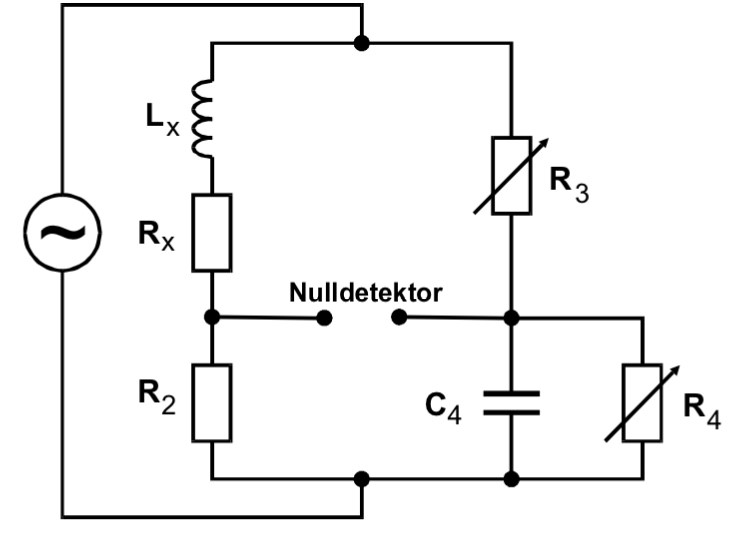
\includegraphics[height=6cm]{data/Schaltung5.jpg}
  \centering
  \caption{Maxwell-Brücke für verlustbehaftete Induktivitäten.}
  \label{fig:Schaltung5}
\end{figure}
\FloatBarrier

\subsection{Wien-Robinson-Brücke}
\label{sec:Theorie5}
Im Gegensatz zu den anderen Brückenschaltungen hängt diese von der Frequenz.
Deshalb wird bei dieser Brückenschaltung die Brückenspannung nicht über Abgleichelemente reguliert, sondern über die Frequenz.
Für Speisespannung und Brückenspannung gilt folgende Beziehung.
\begin{equation}
  \left\lvert \frac{\symbffrak{U}_{\text{s}}}{\symbffrak{U}_{\text{Br}}} \right\rvert^2 = \frac{(\omega^2 R^2 C^2 - 1)^2}{9((1 - \omega^2 R^2 C^2)^2 + 9 \omega^2 R^2 C^2)}
  \label{eqn:gl11}
\end{equation}
Die Brückenspannung verschwindet für $\omega_0 = 1/(RC)$.
Durch die zweckmäßige Einführung von $\Omega = \omega/\omega_0$, lässt sich Gleichung \eqref{eqn:gl11} schreiben als:
\begin{equation}
  \left\lvert \frac{\symbffrak{U}_{\text{s}}}{\symbffrak{U}_{\text{Br}}} \right\rvert^2 = \frac{(\Omega^2 - 1)^2}{9((1 - \Omega^2)^2 + 9 \Omega^2)}
  \label{eqn:gl12}
\end{equation}
Unter reelen Umständen erreicht die Brückenspannung nur ein Minimum > 0, da der Generator auch unerwünschte Oberwellen erzeugt.
Deren Anteil im Vergleich zur Grundwelle wird über den Klirrfaktor beschrieben.
\begin{equation}
  k := \frac{\sqrt{U^2_2 + U^2_3 + ...}}{U_1}
  \label{eqn:13}
\end{equation}
Zur Vereinfachung wird nur eine Oberwelle berücksichtig, die sich mit der Funktion \eqref{eqn:gl12} berechnen lässt:
\begin{equation}
  U_2 = \frac{U_{\text{Br}}}{f(\Omega =2)}
  \label{eqn:14}
\end{equation}
\begin{figure}
  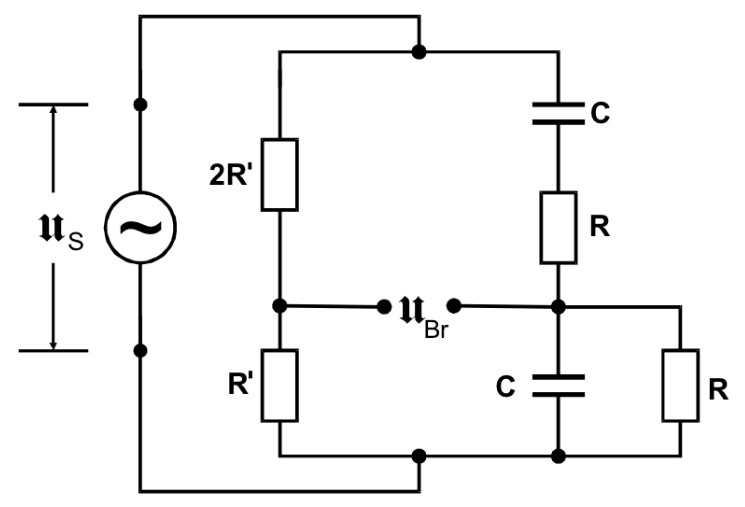
\includegraphics[height=6cm]{data/Schaltung6.jpg}
  \centering
  \caption{Frequenzabhängige Wien-Robinson-Brücke.}
  \label{fig:Schaltung6}
\end{figure}
\FloatBarrier

\subsection{Fehlerrechnung}
\label{sec:Fehlerrechnung}

Alle Mittelwerte werden mit folgender Formel berechnet:
\begin{equation}
  \bar{x} = \frac{1}{N} \sum_{i = 1}^N x_i
  \label{eqn:fehler1}
\end{equation}
Der zugehörige Fehler berechnet sich mit:
\begin{equation}
  \increment \bar{x} = \frac{1}{\sqrt{N}} \sqrt{\frac{1}{N-1} \sum_{i = 1}^N (x_i - \bar{x})^2}
  \label{eqn:fehler2}
\end{equation}
Setzt sich eine Größe aus bereits fehlerbehafteten Größen zusammen, pflanzen diese sich nach der Gauß'schen Fehlerfortpflanzung fort:
\begin{equation}
  \increment f = \sqrt{\sum_{i = 1}^N \left(\frac{\partial f}{\partial x_i} \right)^2 \cdot(\increment x_i)^2}
  \label{eqn:fehler3}
\end{equation}
